% CVPR 2022 Paper Template
% based on the CVPR template provided by Ming-Ming Cheng (https://github.com/MCG-NKU/CVPR_Template)
% modified and extended by Stefan Roth (stefan.roth@NOSPAMtu-darmstadt.de)

\documentclass[10pt,twocolumn,letterpaper]{article}

%%%%%%%%% PAPER TYPE  - PLEASE UPDATE FOR FINAL VERSION
%\usepackage[review]{cvpr}      % To produce the REVIEW version
%\usepackage{cvpr}              % To produce the CAMERA-READY version
\usepackage[pagenumbers]{cvpr} % To force page numbers, e.g. for an arXiv version

% Include other packages here, before hyperref.
\usepackage{graphicx}
\usepackage{amsmath}
\usepackage{amssymb}
\usepackage{booktabs}


% It is strongly recommended to use hyperref, especially for the review version.
% hyperref with option pagebackref eases the reviewers' job.
% Please disable hyperref *only* if you encounter grave issues, e.g. with the
% file validation for the camera-ready version.
%
% If you comment hyperref and then uncomment it, you should delete
% ReviewTempalte.aux before re-running LaTeX.
% (Or just hit 'q' on the first LaTeX run, let it finish, and you
%  should be clear).
\usepackage[pagebackref,breaklinks,colorlinks]{hyperref}


% Support for easy cross-referencing
\usepackage[capitalize]{cleveref}
\crefname{section}{Sec.}{Secs.}
\Crefname{section}{Section}{Sections}
\Crefname{table}{Table}{Tables}
\crefname{table}{Tab.}{Tabs.}


%%%%%%%%% PAPER ID  - PLEASE UPDATE
\def\cvprPaperID{001} % *** Enter the CVPR Paper ID here
\def\confName{[CSED539/AIGS539] Computer Vision}
\def\confYear{2023}


\begin{document}

%%%%%%%%% TITLE - PLEASE UPDATE
\title{B-CARAFE: Better Content-Aware ReAssembly of FEatures}

\author{20220848 Minsu Sun\\
POSTECH CSE\\
{\tt\small minsu.sun@postech.ac.kr}
}
\maketitle

%%%%%%%%% ABSTRACT
\begin{abstract}
CARAFE:Content-Aware ReAssembly of FEatures\cite{CARAFE} has shown improvement on object detection, instance segmentation, semantic segmentation and image inpainting with contextual information injection.
Although CARAFE enables a large receptive field with Kernel Prediction Module, reassembled feature map in manner of content-awareness do actually saturate the region of background beside the the object itself.
We propose B-CARAFE, which is improved approach of CARAFE with adopting activation function in feature reassembly step to suppress the saturation of background in feature map retaining the advantage of performance improvement with negligible additional computation.
\end{abstract}

%%%%%%%%% BODY TEXT
\section{Introduction}
\label{sec:intro}
Content-aware feature reassembly shown by CARAFE\cite{CARAFE} has improved feature reassembly step by adopting kernel prediction module and content-aware reassembly module.
CARAFE clearly showed consistent and substantial gains with negligible computational overhead.
In order to enhance the performance improvement of CARAFE keeping the advantage of negligible computational overhead, aggregating contextual information retaining a large receptive field is critical issue.

\begin{figure}
  \centering
   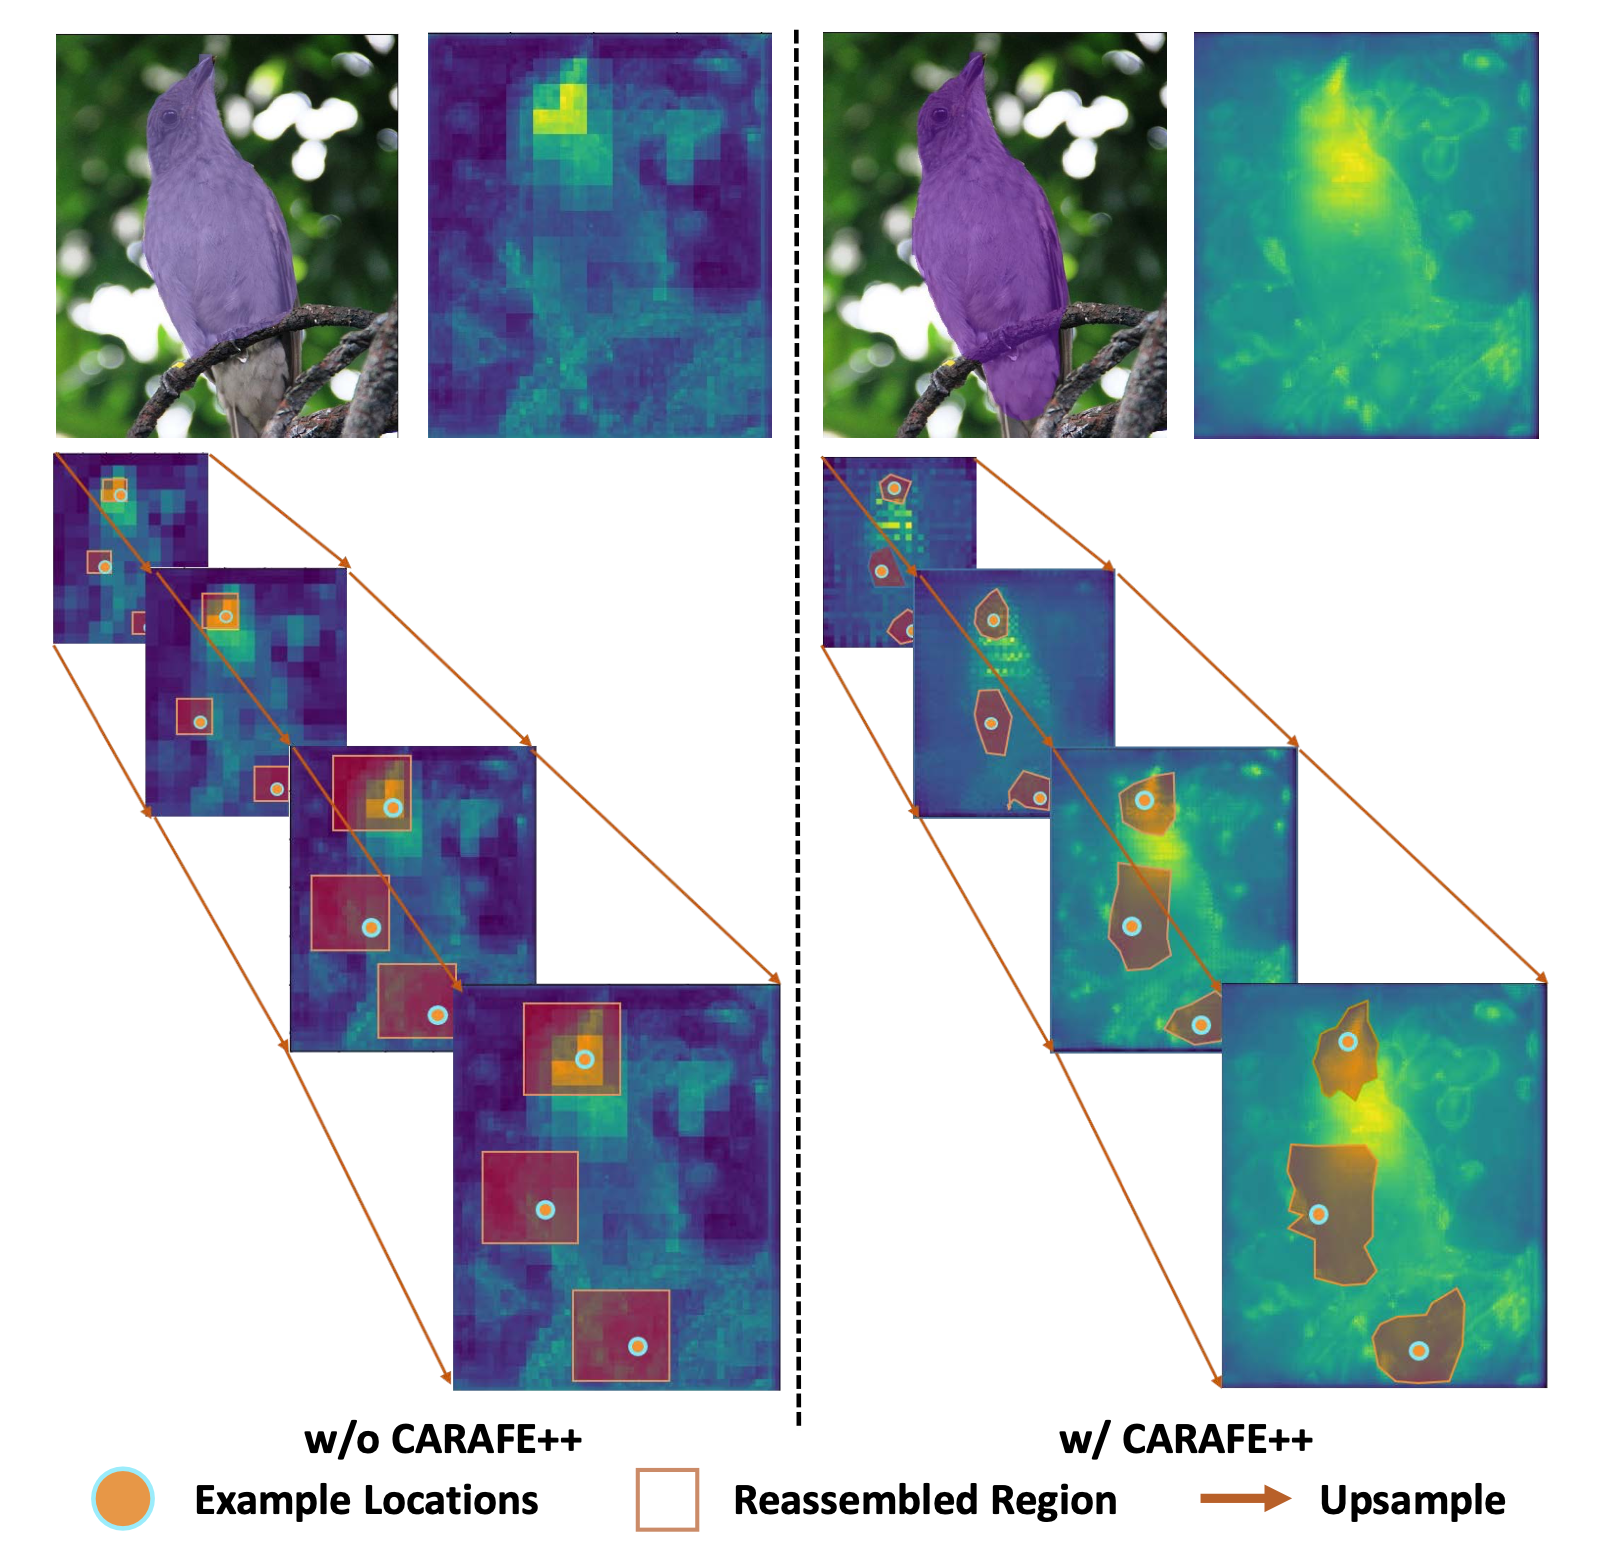
\includegraphics[width=0.8\linewidth]{./img/image.png}
   \caption{\textbf{Comparison of Baseline and CARAFE++\cite{CARAFE}} \textbf{Left}: Multi-level FPN\cite{FPN} features from Mask R-CNN baseline (left to dotted line) and \textbf{Right}: Multi-level FPN features from Mask R-CNN with CARAFE++(right to dotted line).}
   \label{fig:compare_carafe}
\end{figure}

CARAFE used kernel prediction module to extract the contextual information from feature map and content-aware reassembly module to aggregate contextual information to the feature map.
Re-assembled region by CARAFE showed significant improvement compared to the baseline while the background of object is highly saturated compared to the original baseline, which is unwanted result like what \cref{fig:compare_carafe} shows.
To suppress the background saturation beside the object in feature map, we adopt activation functions between levels.
Experimental result shows that adopting B-CARAFE instead of CARAFE showed improvement.

\begin{table*}
  \centering
  \begin{tabular}{@{}cccccccccc@{}}
    \hline
    Method & Backbone & Task & AP & $AP_{50}$ & $AP_{75}$ & $AP_S$ & $AP_M$ & $AP_L$ & FPS \\
    \hline
    Faster R-CNN w/ CARAFE++ & ResNet-50 & BBox & 22.5 & 39.5 & 23.1 & 12.6 & 24.7 & 29.6 & 12.54 fps \\
    Faster R-CNN w/ B-CARAFE(ReLU) & ResNet-50 & BBox & \textbf{21.7} & \textbf{38.9} & \textbf{22.1} & \textbf{13.6} & \textbf{24.3} & \textbf{27.3} & \textbf{13.26 fps} \\
    Faster R-CNN w/ B-CARAFE(GELU) & ResNet-50 & BBox & \textbf{23.7} & \textbf{41.4} & \textbf{24.6} & \textbf{13.2} & \textbf{24.9} & \textbf{30.7} & \textbf{13.25 fps} \\
    \hline
  \end{tabular}
  \caption{Benchmark results on MS COCO 2017}
  \label{tab:result}
\end{table*}

\section{Adopting Activation Function to CARAFE}
\label{sec:formatting}
In order to suppress the background saturation of feature map, it needs to use contextual information for enhancing only objects.

\subsection{Original}
Original structure of CARAFE\cite{CARAFEimpl} does not have any activation function.

\begin{figure}
    \centering
    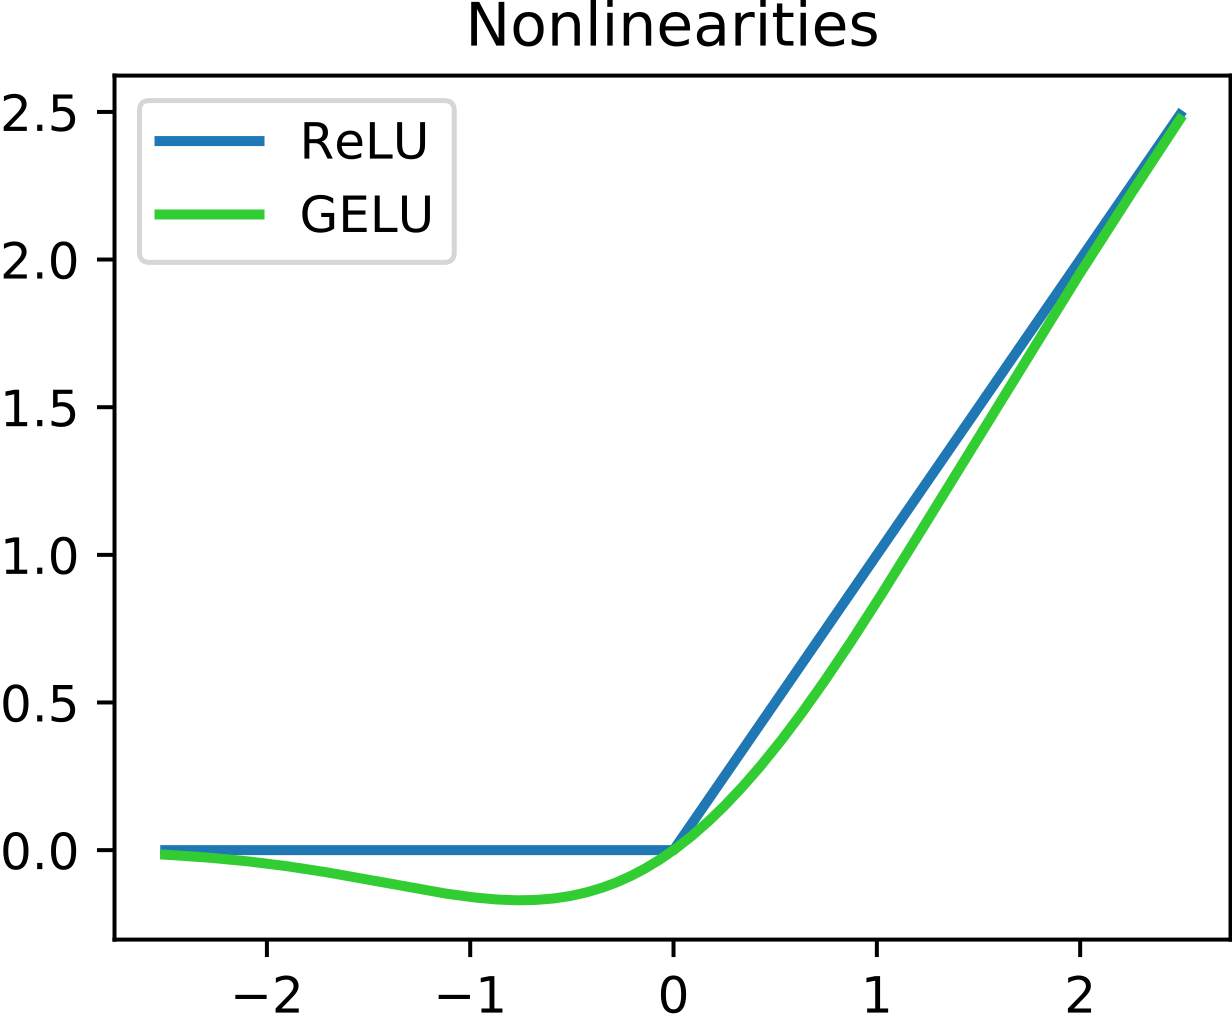
\includegraphics[width=0.8\linewidth]{./img/relu-gelu.png}
    \caption{Comparison of \textbf{ReLU(Rectified Linear Unit)} and \textbf{GELU(Gaussian Error Linear Unit)}}
    \label{fig:relu-gelu}
\end{figure}

\subsection{ReLU(Rectified Linear Unit)\cite{RELU}}
\begin{equation*}
    ReLU(x)=max(0,x)
\end{equation*}
ReLU blocks all signals for negative inputs and releases for positive inputs.
The mechanism for ReLU enables CARAFE to use only object concentrated contextual information.

\subsection{GELU(Gaussian Error Linear Unit)\cite{GELU}}
\begin{equation*}
    GELU(x)\approx\ 0.5x(1+\tanh{[\sqrt{2/\pi}(x+0.044715x^3)]})
\end{equation*}
GELU, the variation of ReLU, releases signals smoothly compared to the ReLU. The mechanism for GELU enables CARAFE to use object concentrated contextual information but with more global context than ReLU does.

\section{Experiments}
\label{sec:formatting}
\subsection{Experiment Details}
\noindent
\textbf{DataSet \& Evaluation Metrics(Object Detection)}
We evaluated B-CARAFE on MS COCO 2017 dataset\cite{COCO}. Results are evaluated with the standard COCO metric, {\em i.e.} AP of IoUs from 0.5 to 0.95.

\noindent
\textbf{Implementation Details}
We evaluated B-CARAFE on Faster R-CNN with the ResNet-50\cite{RESNET} w/ FPN\cite{FPN} backbone. Remaining implementations are specified in MMDetction\cite{CARAFEimpl}.

\subsection{Benchmark Results}
We first evaluate CARAFE++ in Faster R-CNN in object detection as a baseline.

We first replace CARAFE++ with our B-CARAFE(ReLU).
As shown in \cref{tab:result}, B-CARAFE(ReLU) does not improve CARAFE++.

We replace CARAFE++ with out B-CARAFE(GELU) for second experiment.
As shown in \cref{tab:result}, B-CARAFE(GELU) improved CARAFE++ by 1.2\% ({\em i. e. }, from 22.5\% to 23.7\%) on AP.

\section{Conclusion}
We have presented Better Content-Aware ReAssembly of FEatures (B-CARAFE), substantially improved version of CARAFE. It boosts the performance gain trading off negligible additional computation by adopting CARAFE. Adopting well-optimized activation to B-CARAFE will significantly boost up the performance


%%%%%%%%% REFERENCES
{\small
\bibliographystyle{ieee_fullname}
\bibliography{egbib}
}

\end{document}
